\section{Analysis} \label{sec:analysis}

The fine-tuned BERT model's good performance is not surprising, but we could not directly observe how BERT learns to make such predictions. In this section, to explain BERT's performance, we look into the model's hidden layers. We first visualize the model's attention weights before and after training. The weights in each of the 12 attention heads in each of the 12 layers are plotted using the \texttt{bertviz} tool \cite{vig2019transformervis}. We notice that before fine-tuning, the attention heads have several categories of typical patterns, such as attending to the [SEP] symbols or to the next word, as described in e.g. \citet{clark2019does}. However, after fine-tuning, many of these patterns have diluted. Meanwhile, some of the attention heads appear to have learned to attend to the segmentation boundaries. For example, Figure \ref{fig:bert_attention} shows the weights in one attention head in our fine-tuned model. We notice that the model has learned a strong weight for the word ``today", which is the beginning of the introduction in this sequence.


\begin{figure}
  \centering
    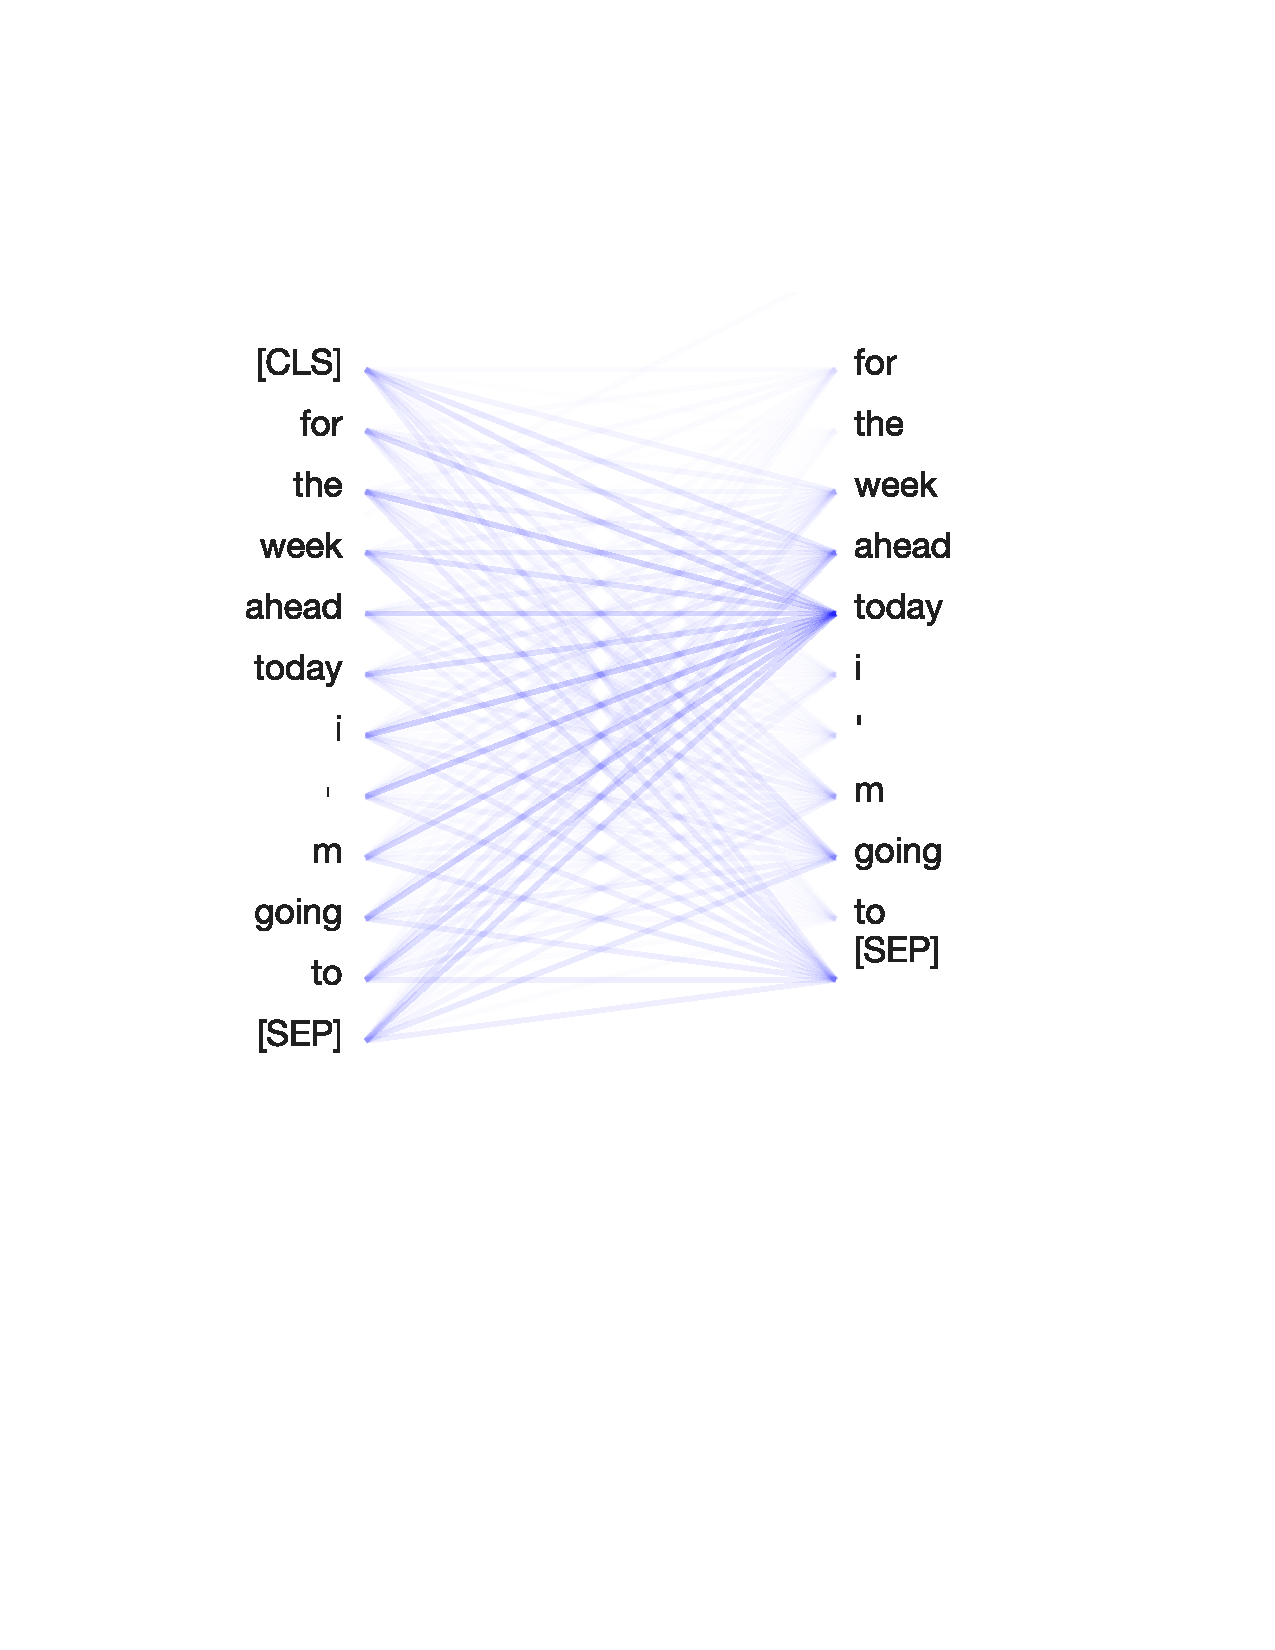
\includegraphics[width=0.48\textwidth]{paper/figs/neuron_view_bert_rm_lines.pdf}
    \vspace{-0.1in}
      \caption{Attention weights of layer 1, head 4 in the fine-tuned BERT model on a sequence extracted from a podcast transcript. Darker lines indicate stronger attention weights. The introduction starts at the word ``today".}
    \label{fig:bert_attention}
\end{figure}

To better understand the information that the model has learned, we further examine the hidden representations that the model learns for the input tokens. We extract the output of each hidden layer as learned vector representations. Inspired by the method used in \cite{van2019does}, we perform a principal component analysis (PCA) on the output vectors, which have 768 dimensions each, for dimensionality reduction. We then plot the tokens using the first two principal components. In this way, we expect to find clusters of tokens that the fine-tuned BERT model consider to be closely related. Figure \ref{fig:bert_layers} shows the token clustering from output of layer 1 and layer 12. We found that in layer 1, words with similar syntactic functions are close to each other; for example, there is a cluster of verbs on the upper left corner and one of auxiliary verbs on the right. Meanwhile, there is no separation between the \texttt{Is-intro} or \texttt{Not-intro} tokens. However, at layer 12, two distinct clusters appear, containing the \texttt{Is-intro} and \texttt{Not-intro} tokens respectively. This is consistent with the findings in \citet{van2019does} and \citet{tenney2019bert}, where the lower and higher layers in BERT are found to contain different types of information. In the lower layers, such as layer 1, the model learns and maintains syntactic representation, while the higher layers focus on task-specific information. We speculate that such learning phrases allow the BERT model the versatility to learn structural information in addition to lexical and topic information.


\begin{figure}
    \centering
    \begin{subfigure}[h]{0.5\textwidth}
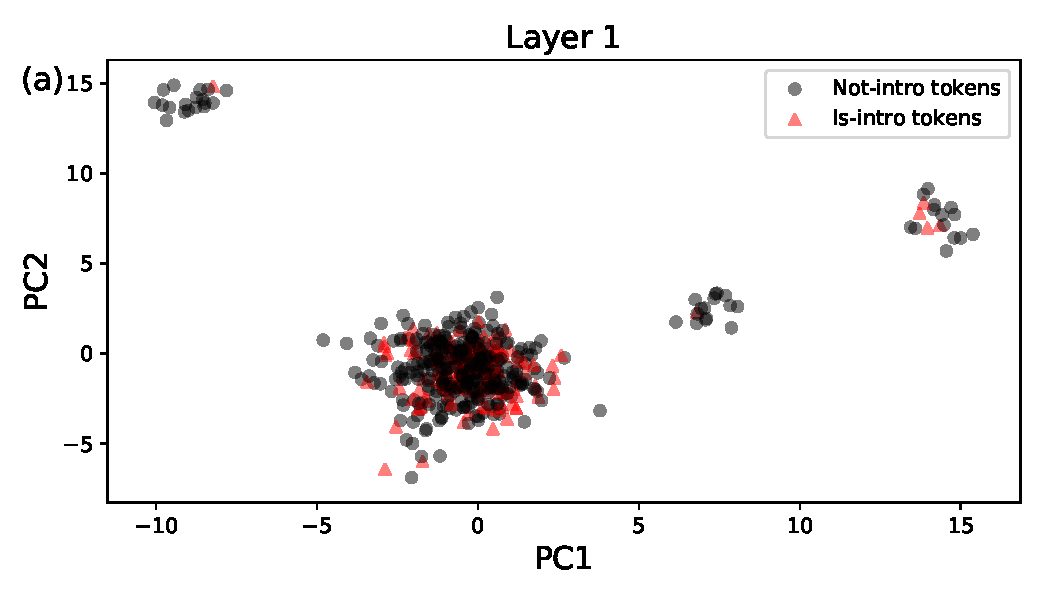
\includegraphics[width=\textwidth]{paper/figs/bert_pca_layer1_sm.pdf}
        % \caption{}
        \label{fig:bert_layer_1}
    \end{subfigure}
    \begin{subfigure}[h]{0.5\textwidth}
        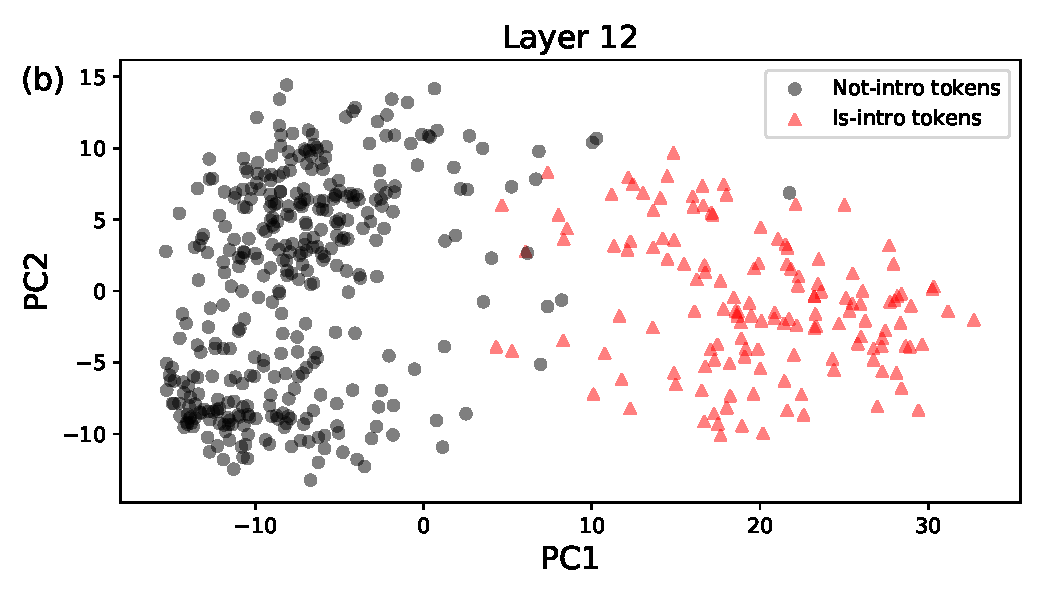
\includegraphics[width=\textwidth, ]{paper/figs/bert_pca_layer12_sm.pdf}
        % \caption{}
        \label{fig:bert_layer_12}
    \end{subfigure}
    \caption{Token clustering from BERT outputs. (a) output of layer 1. (b) output of layer 12. Red markers show the \texttt{Is-intro} tokens, and black show the \texttt{Not-intro} tokens.}
    \label{fig:bert_layers}
\end{figure}
